\documentclass{article}
\usepackage[utf8]{inputenc}
\usepackage[english]{babel}
\usepackage{amsmath}% http://ctan.org/pkg/amsmath
\usepackage{listings}
\usepackage{graphicx}
\usepackage{comment}
\usepackage{float}
\usepackage{biblatex}
\usepackage{lscape}T
\usepackage{csquotes}
\usepackage{multirow}
\addbibresource{bibliography.bib}
\usepackage[a4paper,pdftex,bottom=20mm, width=160mm]{geometry} % A4paper margins
\setlength{\parindent}{0pt} % Tar bort indenteringen på paragrafer
\setlength{\parskip}{1em}

\newcommand{\todo}[1]{\textbf{[TODO: #1]}}

\title{
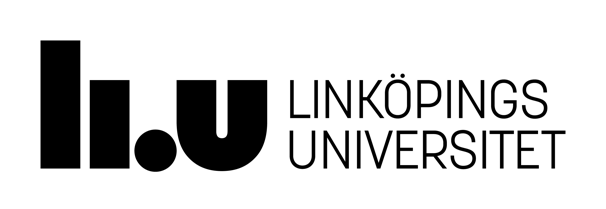
\includegraphics[scale=1.5]{liu_logga.png} \\
\vspace{2.0cm} \textbf{Planning report - The Hive G3 } \\
 \endgraf\rule{\textwidth}{.4pt}
  \large \textbf{TDDE19 Advanced Project Course - AI and Machine Learning}\\
   }


\author{
  \begin{tabular}{ccc}
    Carl Arthur     & Max Eidet       & Oscar Gustafsson \\
    \small carar002 & \small maxei163 & \small oscgu942 \\[1em]
    Jostein Tobias Melaaen & Olle Pettersson & Oskar Schrammel Rask \\
    \small josme010 & \small ollpe910 & \small osksc793 \\
  \end{tabular}
}

\date{\today}

\begin{document}

\maketitle


\newpage
\tableofcontents
\newpage


\section{Introduction}

\subsection{Background}
Small unmanned aerial vehicles (UAVs) are cheap, widely available and hard
to detect, which makes them a growing threat to protected assets such as
infrastructure, bases and public events. Counter-UAS (C-UAS) systems aim to
detect, classify and respond to such drones. A team of autonomous defender
drones guarding an asset can move towards a threat and inspect it at close
range, instead of relying only on fixed sensors. Coordinating such a team
raises a decision problem: which drone should respond to which threat, while
the remaining drones keep the asset covered.
\todo{Add references, e.g.\ from the UAV swarm research in the project vault}

\subsection{Purpose}
The purpose of the project is to develop and evaluate, in simulation, a team
of guard drones that protects an asset. The drones detect, track and
classify incoming drones on their own, while a central decision-maker, the
\emph{hivemind}, decides which drone does what. The project compares a
rule-based hivemind with one trained using reinforcement learning (RL).

\subsubsection{Problem Statement}

The report aims to answer the following questions:
\begin{enumerate}
    \item How can a team of guard drones detect, track and classify a
          hostile drone approaching a protected asset?
    \item How can a central hivemind assign tasks to the drones while
          keeping the asset covered, and does an RL-based hivemind make
          better decisions than a rule-based one?
\end{enumerate}

\subsection{Delimitations}
\begin{itemize}
    \item All work is done in simulation; no physical drones are flown.
    \item Low-level flight control is handled by PX4 and is not developed
          by the group.
    \item The hivemind is centralised. It is a single point of failure;
          a decentralised version is outside the scope.
    \item Enemy drones follow scripted or randomised trajectories and do
          not learn or adapt.
    \item Enemy drones fly at moderate speeds, \todo{e.g.\ 5--10~m/s}, so
          that the thermal detection range gives enough warning (see
          Section~\ref{sec:range}). No radar is used in the main
          implementation.
    \item Battery endurance is not modelled; guard drones can hover
          indefinitely.
    \item The project ends when a threat has been classified.
          \todo{Decide whether interception of a classified enemy is in scope}
    \item The number of drones is limited to \todo{N}, set by what the
          simulation can run.
\end{itemize}

\section{Selected Solutions}
% Which solutions you will investigate, and why.
The system will be developed in simulation using ROS~2, Gazebo and PX4.

\cite{tan2014introduction}

\subsection{Scenario}
\begin{enumerate}
    \item \textbf{Guard.} $N$ drones hover at fixed positions around the
          asset, e.g.\ in a ring. Each watches a sector, and together the
          sectors cover all directions, with some overlap.
    \item \textbf{Detect.} A guard drone detects an unknown object at long
          range with its thermal camera and reports it to the hivemind.
    \item \textbf{Dispatch.} The hivemind sends one drone to investigate.
    \item \textbf{Fill in.} The remaining drones move so that the asset is
          evenly covered again.
    \item \textbf{Approach and track.} The dispatched drone flies towards the
          object and follows it.
    \item \textbf{Classify.} When the object is large enough in the RGB
          image, the drone classifies it with YOLO as enemy, friendly or
          bird.
    \item \textbf{Resolve.} The result is reported to the hivemind. If the
          object is not a threat, the drone returns and the formation is
          restored.
\end{enumerate}

\subsection{System Overview}
PX4 flies each drone, Gazebo simulates the world, the physics and the sensors, and ROS~2 connects them to our code. Each drone runs its own PX4 autopilot. Everything runs in one Docker container, so the same setup works on the group's laptops, whether they run Linux, macOS or Windows, and the Linköpig University lab computers.

The system is split into two levels:
\begin{itemize}
    \item \textbf{Drone level} (one set of nodes per drone): perception,
          tracking, classification and flight. The drone decides
          \emph{how} to carry out an order.
    \item \textbf{Hivemind level} (one node): decides \emph{what} each
          drone should do.
\end{itemize}
The levels communicate through ROS~2 actions. The hivemind sends an order
(\texttt{GUARD}, \texttt{INVESTIGATE}, \texttt{RETURN}); the drone sends
feedback while executing it and a result when done (e.g.\ ``track T7 is an
enemy, confidence 0.92''). Only detections and results are sent to the
hivemind, never images. This interface is fixed early so that both levels
can be developed in parallel; the hivemind is first developed against mock
drones that execute orders directly.

A communication filter node between the levels can add delay, packet loss
and limited range, to study how the system behaves when the link is poor.

\subsection{Drone Level: Detection, Tracking and Classification}
\textbf{Sensors.} Every drone carries the same two forward-facing
cameras, so any drone can be dispatched:
\begin{itemize}
    \item a \textbf{thermal camera} (640$\times$512 pixels, about
          60$^\circ$ field of view) for long-range detection
    \item an \textbf{RGB camera} (1280$\times$720 pixels, about
          65$^\circ$ field of view) for classification at short range.
\end{itemize}
Both are simulated with Gazebo's built-in camera and thermal camera
sensors. The cameras are tilted slightly upwards so that targets appear
against the sky. Guard drones face outwards from the asset; with six to
seven guards the sectors cover all directions with some overlap.

\textbf{Detection.} Detecting a small drone at long range only requires a
few pixels, while classifying it requires many more. A thermal camera is
used for detection because the motors and battery of a drone are warm
against a cold sky, so even a target of 2--3 pixels gives high contrast,
also at night. A 0.5~m drone covers about 3 pixels at 100~m with the
chosen thermal camera. LiDAR is not used: at long range a small drone
typically falls between the beams and gives few or no returns. Each model
in the world is given a temperature (e.g.\ motors about 330~K, birds about
313~K); birds are kept warm on purpose so that they act as realistic false
targets. Since the simulated thermal image is idealised, noise is added in
the detection node. A thermal camera gives bearing but not range; when two
guards see the same object, the hivemind estimates its position by
triangulation.

\textbf{Tracking.} Tracking is done at two levels.

\emph{In the image (on each drone).} Each camera's detections are linked
between frames with ByteTrack: YOLO detections in the RGB image, and
detections of warm spots (temperature threshold and connected pixels) in
the thermal image. ByteTrack uses a Kalman filter to predict where each box
will be in the next frame and also uses low-confidence detections, so a
small target keeps its identity even when it is only detected in some
frames. ByteTrack is built into the YOLO framework used, so it does not
need to be implemented.

\emph{In the world (in the hivemind).} The hivemind tracks every object in
3D in a common frame around the asset, since it needs to know where the
object is and where it is heading. Each track is estimated with a Kalman
filter with a constant-velocity model, where the state is position and
velocity, $\mathbf{x} = [x, y, z, v_x, v_y, v_z]^T$. In the
\emph{prediction} step the object is assumed to keep its velocity and the
uncertainty grows, by an amount set by the process noise $Q$ that models
how much the object can manoeuvre. In the \emph{update} step each new
measurement is weighted against the prediction according to its
measurement noise $R$. The filter gives a smooth position and an estimate
of the velocity from noisy and irregular measurements. The velocity is
used to estimate when a threat reaches the asset, and lets the dispatched
drone fly to where the object will be rather than where it was.

A camera measures direction (azimuth and elevation) but not range. Two
approaches are used, in order:
\begin{enumerate}
    \item \textbf{Triangulation and linear Kalman filter.} When two guards
          see the same object, the intersection of their lines of sight
          gives a position, which is used as the measurement in a linear
          Kalman filter. This is simple, but requires two drones to see
          the object at the same time.
    \item \textbf{Extended Kalman filter (EKF).} The directions are used
          directly as measurements, which works also when only one drone
          sees the object: as the dispatched drone moves, lines of sight
          from different positions make the range observable
          (bearing-only tracking). When YOLO has found the target, the
          size of its box gives a rough range as well, since the size of
          a drone is approximately known.
\end{enumerate}

Several objects are handled with a global nearest neighbour tracker. Each
new measurement is compared with the predicted position of every track,
taking the uncertainty into account (Mahalanobis distance); measurements
too far from a track are rejected (gating), and the remaining
measurements are assigned to tracks with the Hungarian method. A
measurement that does not match any track starts a new track with status
\texttt{TENTATIVE}; it becomes \texttt{CONFIRMED} after e.g.\ 3 hits in 5
updates, and only then is it acted upon by the hivemind. A track that is
not updated for some time becomes \texttt{LOST}. More advanced trackers
(JPDA, MHT) are not needed for the small number of objects in the
scenarios. Kalman filter and EKF implementations are available in the
Python library \texttt{filterpy}.

\emph{Thermal and RGB camera in the same track.} Both cameras feed the same
world track. The thermal cameras on the guards create the track at long
range; when the dispatched drone's RGB camera finds the target, its
measurement falls within the gate of the existing track, so the object
keeps its identity and is updated from unknown to classified instead of
appearing as a new object. Each sensor has its own measurement noise $R$:
the thermal camera has coarser pixels (about 1.6~mrad compared to
0.9~mrad for the RGB camera) and therefore gets less weight per
measurement. On the dispatched drone the two cameras also work together:
since their relative mounting is known, a warm spot in the thermal image
can be mapped to a region of the RGB image, and YOLO can be run on an
enlarged crop of that region, which lets it find the target at a longer
range than when it searches the whole image.

\textbf{Classification.} The thermal image has too low resolution for
reliable classification, so classification uses the RGB camera, where a
0.5~m drone covers about 22 pixels at 25~m. YOLO runs onboard the
dispatched drone, in that drone's perception node, and only that drone
processes its RGB images. Running it onboard avoids streaming video to a base
station, gives low latency for following the target, and keeps working if
the link to the hivemind is jammed. A small model (e.g.\ nano size) is used
so the choice is realistic for drone hardware.

The model is trained in two steps, starting from YOLO weights pretrained on
COCO, which already include a bird class. First it is fine-tuned on the
Seraphim drone detection dataset, about 83\,000 images of drones collected
from 23 open datasets, already in YOLO format and licensed under CC~BY~4.0.
This teaches the model what real drones look like in many settings.
Second, it is fine-tuned on images generated in Gazebo, where ground truth
gives labels automatically and enemy, friendly and bird use different 3D
models, so that the model learns the project's own classes. Birds are
included in the Gazebo images so that the model does not forget them. If
more data is needed, the synthetic SynDroneVision dataset (CC~BY~4.0) or
the real DUT Anti-UAV dataset can be added. The distance at which classification becomes
reliable is measured, not assumed.

\subsection{Discussion: Realism of the Detection Range}\label{sec:range}
The thermal camera detects a small drone at roughly 100--200~m. In a real
attack this is too short. A fast attack drone can fly at 30--50~m/s, which
means that it covers 150~m in about 3--5~seconds, and even a slower
commercial quadcopter at 15~m/s needs only about 10~seconds. In that time
the system must confirm the detection, the hivemind must decide which drone
to send, and the dispatched drone must fly close enough (about 25~m) to
classify the target. The guard drones are also slower than a fast attacker,
so in practice the threat would reach the asset before it has been
classified. \todo{Add reference for typical attack drone speeds}

A realistic C-UAS system would therefore not rely on cameras for the first
detection. It would use a ground-based radar at the asset that detects
small drones at several hundred metres or more, and gives range and
velocity directly, without triangulation. At 1~km a drone flying at 30~m/s
gives about 30~seconds of warning, which leaves time for a decision and an
inspection. In such a system the radar provides the early warning and the
direction, and the cameras on the drones are used to confirm and classify
the target at short range, which is where they are strongest. Radar has
weaknesses of its own: small drones have a small radar cross-section and
are easily confused with birds, which is one reason why camera-based
classification is still needed.

In this project the radar is left out of the main implementation, since
Gazebo has no radar sensor and the focus is on the drones' own perception
and on the hivemind. To keep the scenario meaningful, the enemy drones are
given speeds that leave time to react with the thermal detection range.
For the hivemind, what matters is the ratio between the warning time and
the time it takes to respond, not the absolute distances, so the decision
problem is the same as in a radar-supported system with longer distances
and faster threats. If time allows, a simulated radar node (true position
with noise, range-dependent detection probability and false alarms) can be
added to show how the earlier warning changes the hivemind's decisions.

\subsection{Hivemind Level}
\textbf{World model.} The hivemind keeps tables of tracks (position,
velocity, status, label), drones (position, state, current order) and
orders (status), together with a timestamped event log. The log records
every detection, decision and result, so that decisions can be explained
and evaluation metrics computed afterwards.

\textbf{Decision loop.} Several times per second the hivemind updates its
tracks and drone states, ranks threats (distance to the asset, heading,
speed, classification), assigns drones to threats, computes new guard
positions for the remaining drones, and monitors running orders, reassigning
them on failure or timeout.

\textbf{Rule-based hivemind (baseline).} The nearest free drone investigates
the highest-ranked unclassified track; the remaining drones spread evenly
on the ring; at most $k$ drones may be away at the same time.

\textbf{RL-based hivemind.} The RL policy replaces the assignment and
coverage decisions. With one threat at a time the rule-based choice is
nearly optimal, so RL is only expected to help in harder scenarios: several
simultaneous threats, decoys meant to pull guards away, and birds or
friendly drones that waste resources. A hybrid, where RL scores each
(drone, track) pair and a solver makes the assignment, is considered if a
pure RL policy is unstable. \todo{Choose algorithm, e.g.\ PPO}

\textbf{Training in a fast simulator.} Training the hivemind in PX4 +
Gazebo is too slow: every drone needs its own PX4 instance, the simulation
runs near real time, and resets are slow. Since the hivemind only makes
abstract decisions, it is trained in a fast Python simulator (Tier~1) where
drones move at constant speed towards their goals and detection and
classification succeed with given probabilities. These probabilities,
flight times and classification distances are measured in Gazebo with the
real drone level (calibration) and randomised slightly during training.
The simulator follows the Gymnasium/PettingZoo interface, so standard RL
libraries can be used, and training runs in parallel on the supercomputer.
The trained policy is then evaluated in PX4 + Gazebo (Tier~2) through the
same order interface.

\section{Evaluation}
The rule-based and RL-based hivemind are evaluated in Gazebo on the same
scenarios, with many random seeds per scenario. Results are reported as
mean and spread.
\begin{itemize}
    \item \textbf{Scenarios:} single threat; several simultaneous threats;
          decoy followed by an attack from another direction; birds and
          friendly drones; degraded communication.
    \item \textbf{Drone-level metrics:} detection range, missed and false
          detections, tracking error, classification accuracy and the
          distance at which it becomes reliable, inference time.
    \item \textbf{Hivemind metrics:} time from detection to
          classification, share of the perimeter covered over time (and its
          minimum), closest approach of an enemy to the asset, enemies
          reaching the asset, drones sent to non-threats.
\end{itemize}
All runs are logged with rosbag2 and the hivemind event log, so they can be
replayed and analysed.

\section{Time Plan}
\todo{Replace week numbers with calendar weeks and course deadlines}

\begin{table}[H]
\centering
\begin{tabular}{|l|l|p{8.5cm}|}
\hline
\textbf{Weeks} & \textbf{Phase} & \textbf{Activities} \\ \hline
1--2 & Environment and interfaces &
  Shared Docker environment, several drones with namespaces in offboard
  mode, order interface (ROS~2 actions), mock drones, test run on the
  supercomputer. \\ \hline
3--4 & Drone level &
  Drone model with thermal and RGB camera, temperatures in the world,
  guard behaviour, thermal detection, tracking and following, scripted
  enemy drone, YOLO dataset from the RGB camera. \\ \hline
3--5 & Rule-based hivemind &
  World model, decision loop and rules; developed against mock drones,
  then run in Gazebo. \\ \hline
5--6 & Integration &
  Onboard YOLO classification, full scenario with rule-based hivemind,
  calibration measurements. \\ \hline
6--8 & RL hivemind &
  Tier~1 simulator, training on the supercomputer, transfer to Gazebo. \\ \hline
9--10 & Evaluation and report &
  Batch evaluation of both hiveminds, analysis, final report and
  presentation. \\ \hline
\end{tabular}
\caption{Preliminary time plan.}
\end{table}

\subsection{Milestones}
\begin{table}[H]
\centering
\begin{tabular}{|l|l|p{9.5cm}|}
\hline
\textbf{ID} & \textbf{Week} & \textbf{Milestone} \\ \hline
M1 & 2  & All members run the shared environment; several drones fly in
          offboard mode; order interface agreed. \\ \hline
M2 & 4  & A guard drone detects, tracks and follows an enemy drone. \\ \hline
M3 & 6  & Full scenario runs with the rule-based hivemind and onboard YOLO. \\ \hline
M4 & 8  & RL hivemind trained in Tier~1 and running in Gazebo. \\ \hline
M5 & 10 & Evaluation complete; final report submitted. \\ \hline
\end{tabular}
\caption{Milestones.}
\end{table}

\section{Work Distribution}
\begin{table}[H]
\centering
\begin{tabular}{|l|l|}
\hline
\textbf{Area} & \textbf{Responsible} \\ \hline
Environment, simulation and integration & \todo{name} \\ \hline
Detection and tracking                  & \todo{name} \\ \hline
YOLO dataset and classification         & \todo{name} \\ \hline
Hivemind: world model and rules         & \todo{name} \\ \hline
Tier~1 simulator and RL training        & \todo{name} \\ \hline
Evaluation and report                   & \todo{name} \\ \hline
\end{tabular}
\caption{Areas of responsibility.}
\end{table}

\section{Risks}
\begin{table}[H]
\centering
\begin{tabular}{|p{6.5cm}|p{8.5cm}|}
\hline
\textbf{Risk} & \textbf{Mitigation} \\ \hline
PX4 + Gazebo too heavy for many drones &
  Fix the maximum number of drones in weeks 1--2; run large scenarios on
  the supercomputer. \\ \hline
Small drones hard to detect at long range &
  Thermal camera for detection; YOLO on RGB only at short range; simulated
  radar node as fallback. \\ \hline
Simulated thermal image too idealised &
  Add noise and warm false targets (birds); measure detection range in a
  test before relying on it. \\ \hline
Two cameras per drone too heavy to render &
  Low frame rate; process RGB only on the dispatched drone. \\ \hline
YOLO too slow on CPU (no GPU in Docker on Mac) &
  Small model; run YOLO only on the dispatched drone and a few times per
  second; heavy runs on a GPU machine. \\ \hline
RL does not beat the rule-based hivemind &
  Design scenarios where rules fail (several threats, decoys); the
  comparison is a valid result either way. \\ \hline
Reward hacking, e.g.\ never dispatching to keep coverage &
  Reward both coverage and classified threats; inspect the event log. \\ \hline
Policy does not transfer from Tier~1 to Gazebo &
  Calibrate Tier~1 against Gazebo; randomise its parameters. \\ \hline
Members blocked by each other &
  Fix the order interface early; mock drones for the hivemind. \\ \hline
Docker not allowed on the supercomputer &
  Run the same image as an Apptainer container. \\ \hline
\end{tabular}
\caption{Identified risks and mitigations.}
\end{table}

\newpage
\printbibliography

\end{document}